\chapter{p3 = 9 (1 graphs)}
\newpage\begin{figure}
  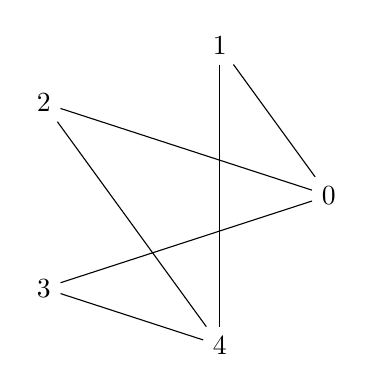
\begin{tikzpicture}
      \draw
        (0.0:2) node (0){0}
        (72.0:2) node (1){1}
        (144.0:2) node (2){2}
        (216.0:2) node (3){3}
        (288.0:2) node (4){4};
      \begin{scope}[-]
        \draw (0) to (1);
        \draw (0) to (2);
        \draw (0) to (3);
        \draw (1) to (4);
        \draw (2) to (4);
        \draw (3) to (4);
      \end{scope}
    \end{tikzpicture}
\end{figure}
\begin{itemize}
\item signature: 1110001011
\item g: Graph with 5 nodes and 6 edges
\item order: 5
\item size: 6
\item max degree: 3
\item degrees: 2,2,2,3,3
\item is tree: 0
\item is bipartite: 1
\item has bridge: 0
\item is chordal: 0
\item is complete: 0
\item min cycle basis weight: 8
\item min cycle basis size: 2
\item diameter: 2
\item radius: 2
\item is eulerian: 0
\item is planar: 1
\item number of faces: 3
\item is regular: 0
\item p3: 9
\item p4: None
\item property hash: 3f4bcf5a4ec237e2552744d521bf79165642d68a302f95462c79464742d0208f
\end{itemize}
\newpage
